\documentclass{report}
\usepackage[english]{babel}
\usepackage[utf8]{inputenc}
\usepackage[T1]{fontenc}
\usepackage{listings}
\usepackage{titlesec}
\usepackage{color}
\usepackage{graphicx}

\titleformat{\chapter}[display]
            {\normalfont\bfseries}{}{0pt}{\Huge}

\lstset{ escapeinside={(*}{*)} }

\title{Méthodes et Outils pour la Conception Avancée}
\author{Castel Antonin, Reboul Paul, Vandendorpe Thomas}
\begin{document}
\maketitle{}
\tableofcontents

\chapter{Introduction}

Ce dossier rassemble les travaux effectués lors du cours de ``Méthodes et Outils pour la Conception Avancée''. L'objectif ici, est de montrer les bonnes pratiques à avoir lors de la conception d'un programme. Nous illustrerons ces bonnes pratiques à partir de l'exemple d'un programme de puissance 4 (en langage C), initialement codé de façon peu rigoureuse, que nous tenterons d'améliorer tout au long de ce dossier. Par améliorer, on entend  la maintenabilité, la réutilisabilité et la documentation du code, la qualité et la couverture des tests, la détection de défauts et d'erreurs, l'analyse et l'amélioration des performances, ainsi que l'analyse de la vulnérabilité à certaines attaques. Nous expliquerons les différentes méthodes et outils permettants ces améliorations...

\chapter{Modularité, maintenabilité, réutilisabilité}
\section{Titre}
...
\section{Titre}
...

\chapter{Qualité des tests}
On ne peut pas parler de qualité du logiciel sans parler des tests. Bien que ne prouvant pas l'absence de bug dans un code, les tests exécutés sur un programme sont de bons indicateurs sur sa qualité. Il est nécessaire de ``penser tests'' tôt dans la création d'un logiciel, car les tests sont écrits au fur et à mesure de la conception et sont destinés à être exécutés plusieurs fois, ceci afin de vérifier que les modifications et ajouts dans le code permettent toujours de valider les tests précédents. Et ceci est d'autant plus vrai lors d'un projet en équipe où les modifications des uns peuvent affecter les modifications des autres. Nous allons dans cette partie présenter deux méthodes permettant d'assurer une certaine rigueur dans les tests: l'une au sujet des tests unitaires et la seconde concernant l'analyse de couverture.
\section{Les tests unitaires}
Les tests unitaires sont des tests s'appliquant à une partie d'un programme et permettant de vérifier le programme par bloc. Un bloc de programme est en faite une fonction, et l'idée est d'écrire un test qui appelle une certaine fonction avec certains paramètres (judicieusement choisis si possible, c'est à dire couvrant le plus de branches possibles) et de vérifier que le résultat renvoyé par la fonction est bien le résultat attendu. Il est possible d'écrire ces tests en suivant un processus de développement dirigé par les tests, qui consiste à écrire les tests avant d'écrire la fonction correspondante. Mais on peut également les écrire si on dispose déjà de la fonction à tester en utilisant sa spécification (qui devrait être facilement accessible si le code a été documenté avec un outil adéquat), ce qui arrive si l'on est amener à retoucher un code existant.

TODO: Nécessiter de prendre en compte/modifier des fonctions pour permettre le test unitaire (valeur retour etc...) + decoupage code en fonction
\subsection{Exemple de test}
Illustrons ce principe de tests unitaire à l'aide d'un exemple tiré d'un programme de puissance 4 (en langage C). Nous souhaitons écrire un test pour la fonction suivante:

\begin{scriptsize}
\begin{lstlisting}

int checkfull(Board board);

/*
*Verifie si une grille(Board) est pleine
*
*Parameters
*   board: une table de jeu
*
*Returns
*   0 si la grille est pleine, 1 sinon
*/


\end{lstlisting}
\end{scriptsize}

Il existe de nombreux frameworks permettant l'automatisation des tests unitaires, dans cet exemple, on utilise CuTest. Il peut être intéressant de remarquer (en gras) l'assignation des variable actual (valeur renvoyé par la fonction testée), de  expected (valeur attendue) et leur comparaison (qui fonctionne un peu comme une assertion).
\begin{scriptsize}
\begin{lstlisting}

void Test_checkfull(CuTest *tc){
  int i,j,expected,actual;
  Board b=boardVide(15,22);
  for(i=0;i<b.height;i++){
    for(j=1;j<=b.width;j++){
      (*\bfseries actual = checkfull(b);*)
      (*\bfseries expected = 1;*)
      (*\bfseries CuAssertIntEquals(tc, expected, actual);*)
      board_put(&b,j);
    }
  }
   (*\bfseries actual = checkfull(b); *)
   (*\bfseries expected = 0; *)
   (*\bfseries CuAssertIntEquals(tc, expected, actual); *)
}

\end{lstlisting}
\end{scriptsize}

Les tests écrits de cet façon pourrons ensuite tous être exécuter en même temps et des informations sur les échecs des tests seront disponibles:


\begin{lstlisting}

.......F.........

There was 1 failure:
1) Test_checkfull: src/CuTestTest.c:221: expected <0> but was <1>

!!!FAILURES!!!
Runs: 17 Passes: 16 Fails: 1

\end{lstlisting}
\begin{lstlisting}

.................

OK (17 tests)
\end{lstlisting}

Comme les tests sont ensuite facile à relancer, il est important de les réexécuter à chaque changement important dans le code afin d'évité la régression.

\subsection{Couverture}
La couverture est un indicateur permettant de savoir quelles parties du code ont été couvertes par les tests. Utiliser la couverture seule n'est pas forcément intéressant, puisqu'elle n'indique pas si les tests ont été validés ou non. En revanche, en combinaison des tests unitaire vu précédemment, on a un indicateur de la qualité des tests très puissant puisqu'on a l'information du pourcentage du code tester et du nombre de tests validés.
\subsection{Exemple de couverture}
Nous avons utilisé l'outil gcov afin d'observer la couverture de notre puissance 4. Comme ce dernier ne donne qu'un résultat textuel de la couverture, nous avons complété son utlisation avec l'outil lcov, qui utilise ce que gcov a produit mais rajoute une interface html afin que la couverture soit plus facile à lire. On peut ainsi observer le pourcentage de lignes/fonctions visitées par les tests:

\begin{center}
  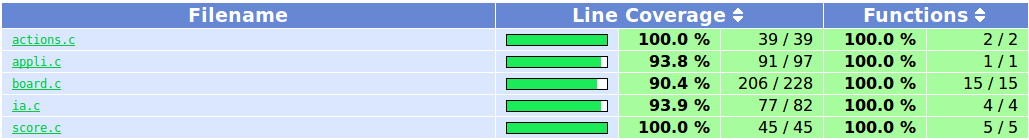
\includegraphics[width=13cm]{couverture1.png}
\end{center}

En plus des pourcentage de couverture, on peut également directement voir sur le code ce qui a été couvert(en bleu) et ce qui ne l'a pas été(en rouge). Cela est pratique lorsqu'on écrit des tests en essayant de passer par le plus de branches possibles (conditions,boucles,...) du programme.

\begin{center}
  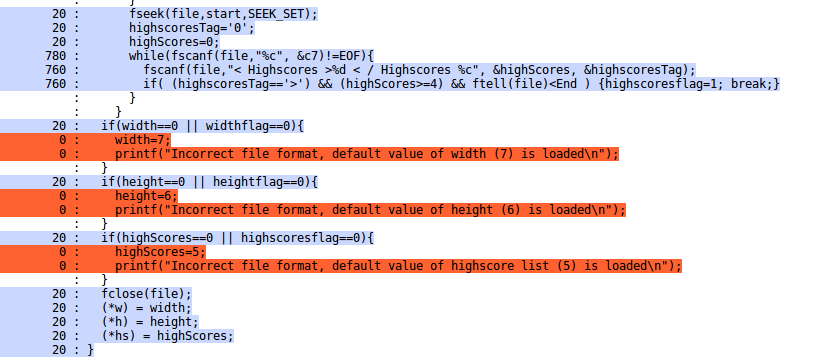
\includegraphics[width=13cm]{couverture2.png}
\end{center}

\end{document}
